\chapter{Pildepon}
%
% - Purpose & Problem description:
%     These first two parts give reader short details about the test case,
%     the physical phenomena involved and specify how the numerical solution will be validated
%
\section{Description of the problem}
This test case shows that \telemac{2d} is able to represent the impact of an obstacle on a channel flow : it simulates a laminar and very viscous flow in a channel with two cylindrical piers. \\
The channel is 28.5 m long and 20 m wide (L=28.5~m and H=20~m) with two bridge piers positioned at $P_1=(-5,4)$, $P_2=(-5,-4)$ and a diameter D of 4~m.
The geometry is shown in the Figure \ref{fig:geo:bridge}.
\begin{figure}[H]
 \centering
 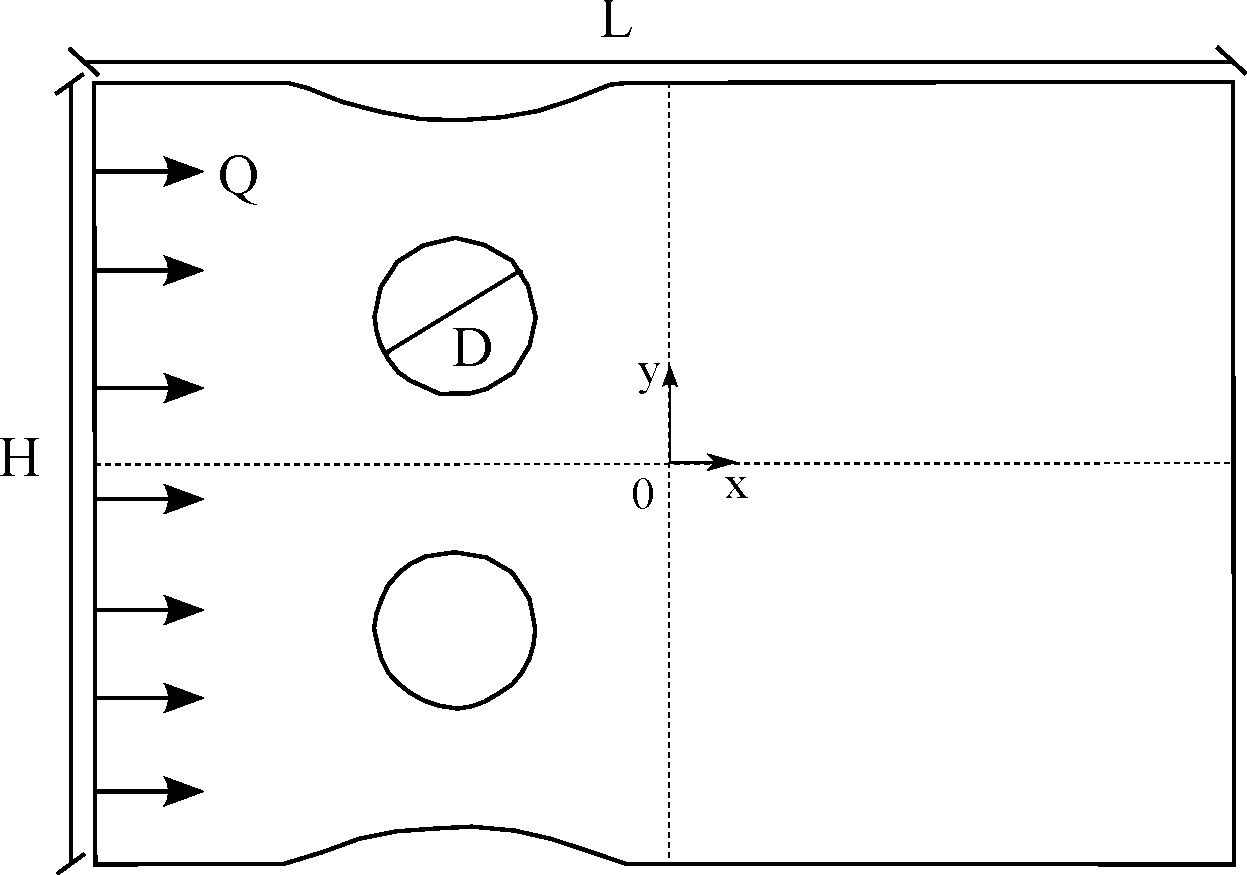
\includegraphics[scale=0.3]{img/geometry.pdf}
 \caption{Geometry of the pildepon test case.}
 \label{fig:geo:bridge}
\end{figure}
The section is trapezoidal (see the bottom in the Figure \ref{fig:bott:bridge}) and the minimum value of the bottom elevation is equal to -4~m in the main channel.
The bottom friction is described by the Strickler law with a coefficient equal to $k_s=40~\text{m}^{1/3}\text{s}^{-1}$.
\begin{figure}[H]
 \centering
 \includegraphicsmaybe{[scale=0.25]}{../img/bathy.png}
 \caption{Topography at the inlet of the channel.}
 \label{fig:bott:bridge}
\end{figure}
At the inlet of the channel, we gradually impose as upstream boundary condition a flow discharge Q = $62~\text{m}^3\text{s}^{-1}$,
while at the outlet a null free surface is imposed, which is also the initial condition. On the lateral walls and on the cylinder, slip boundary conditions are imposed.
The fluid considered presents a kinematic viscosity $\nu=0.021~\text{m}^2\text{s}^{-1}$. The average flow velocity in the upstream undisturbed field is
about $U$ = 0.95~m/s. Taking into account the diameter of the cylindrical pier, the Reynolds number is $Re = UD/\nu=180$. \\
For this case, neither analytical nor experimental solutions are available, but the formation of von Karman vortex is expected behind the piers. The validation is performed computing the Strouhal number for the two piers, given by the following formula:
\begin{equation*}
St=\frac{f_{lift}D}{U}
\end{equation*}
where $f_{lift}$ is the lift frequency which usually corresponds to the vortex shedding frequency, D is the diameter of the cylinder and U is the average free-stream velocity.
%Due to the alternating vortex wake the oscillations in lift force occur at the vortex shedding frequency and oscillations in drag force occur at twice the vortex shedding frequency.
In order to compute the lift frequency, a FFT (Fast Fourier Transform) has been performed on the signal which describes the variation of the force with time. The force is computed as:
\begin{equation*}
F=\int_0^l\int_0^h \rho~gz \vec{n}~dz~ds
\end{equation*}
where $\rho$ is the water density, $g$ is the acceleration of gravity and $\vec{n}$ is the normal vector. The integral is performed on the cylinder with boundary $l$ and along the vertical direction $z$. \\
To perform an appropriate analysis on several cycles, the simulation time is set to 1200~s. \\
Finally, in order to check the mass coservation of the advection schemes of \telemac{2d}, a tracer is released at the inlet with the following boundary condition:
\begin{equation*}
 c(x=-13.5,y)=\left\{
\begin{array}{rl}
 2 ~g/l\quad & \text{if} \quad H/2-9~\leq \text{y} \leq H/2-8\\
 1 ~g/l\quad & \text{otherwise}
\end{array}\right .
\end{equation*}
A free condition is imposed at the outlet. The error on the mass is computed as follows:
\begin{equation*}
  \epsilon_{M}= M_{start}+M_{in}-M_{end}
\end{equation*}
M$_{\text{start}}=\int_{\Omega}(hc)^nd\Omega$ is the mass at the beginning of the simulation,  M$_{\text{end}}=\int_{\Omega}(hc)^{n+1}d\Omega$ is the mass at the end of the simulation, M$_{\text{in}}=\int_{\Gamma}hc\vec{u}\vec{n}d\Gamma$ is the mass introduced (and leaved) by the boundaries; where $\Omega$ is the computational domain and $\Gamma$ is its boundary.
The realtive error is computed as:
\begin{equation*}
  \epsilon_{rel}=\frac{\epsilon_{M}}{\max(|M_{start}|,|M_{in}|,|M_{end}|)}
\end{equation*}
\section{Numerical parameters}
The computational domain is made up by 4304 triangular elements and 2280 nodes and it is shown in Figure \ref{fig:mesh:bridge}.
\begin{figure}[H]
 \centering
 \includegraphicsmaybe{[scale=0.45]}{../img/Mesh.png}
 \caption{Mesh of the channel with two cylindrical piers.}
 \label{fig:mesh:bridge}
\end{figure}
Three different numerical configurations are tested: \\
\textbf{CASE A}
\begin{itemize}
 \item Equations: Saint-Venant FE
 \item Type of element:
 \begin{itemize}
  \item Linear P1 for velocities
  \item Linear P1 for water depth
 \end{itemize}
 \item Advection scheme for velocities: weak characteristics with 12 Gauss points
 \item Linear system: wave equation
 \item Time step: 0.8~s
 \item Solver: conjugate gradient with accuracy $10^{-5}$
\end{itemize}
\textbf{CASE B}
\begin{itemize}
 \item Equations: Saint-Venant FE
 \item Type of element:
 \begin{itemize}
  \item Quadratic P2 for velocities
  \item Linear P1 for water depth
 \end{itemize}
 \item Advection scheme for velocities: strong characteristics
 \item Linear system: primitive equations
 \item Time step: 0.1~s
 \item Solver: GMRES with option 1 and accuracy $10^{-5}$
\end{itemize}
\textbf{CASE C}
\begin{itemize}
 \item Equations: Saint-Venant FV
 \item Finite volume scheme: kinetic order 2
 \item Time step: variable with CFL=0.9
\end{itemize}
For the tracer, all the advection schemes of \telemac{2D} are tested in the configuration A.
In the case of the predictor-corrector schemes, the number of corrections is set to 5; for the LIPS schemes, the number of sub-steps is equal to 10 and the accuracy for diffusion of tracers is set to $10^{-10}$. It is important to note that the last parameter is used even if the keyword \telkey{DIFFUSION OF TRACERS} is set to NO. Indeed, when using the LIPS schemes, a linear system has to be solved and this parameter defines the accuracy of the solver.
% - Results:
%     We comment in this part the numerical results against the reference ones,
%     giving understanding keys and making assumptions when necessary.
%
%
\section{Results}
Table \ref{t2d:bridge:tab1} contains the Strouhal number obtained for the different numerical configurations.
\begin{table}[H]
\centering
\caption{Pildepon test case: Strouhal number for the upper and lower piers according to the different numerical configurations.}
\begin{tabular}{l|}
\\ \hline CASE A \\ CASE B \\ CASE C
\end{tabular}%
\begin{tabular}{c|c}
  Strouhal for upper pier & Strouhal for lower pier \\
\hline
\InputIfFileExists{../img/table.txt}{}{}
\label{t2d:bridge:tab1}
\end{tabular}
\end{table}
The results are reasonable for the various configurations.\\
Table \ref{t2d:bridge:balance} shows the mass balance at the end of the simulation according to the different advection schemes
It can be noted that only the characteristics are not mass conservative.
\begin{table}[H]
\centering
\caption{Pildepon test case: mass balance for the different advection schemes.}
\begin{tabular}{l|}
\\ \hline Strong Char. \\ N  \\ N PC1 \\ N PC2 \\ PSI \\ PSI PC1 \\ PSI PC2 \\ PSI LIPS \\ NERD
\end{tabular}%
\begin{tabular}{c|c|c|c|c}
   M$_{\text{start}}$&  M$_{\text{end}}$ & M$_{\text{in}}$ & $\epsilon_{M}$ & $\epsilon_{rel}$\\
\hline
\InputIfFileExists{../img/massb_A.txt}{}{}
\label{t2d:bridge:balance}
\end{tabular}
\end{table}

